% -*- TeX -*- -*- UK -*- -*- BMR -*-
% ----------------------------------------------------------------
% Beamer presentation ************************************************
%
% Subhaneil Lahiri's template
%
% To compile:
%   Ctrl-Shift-P
%
% **** -----------------------------------------------------------
\documentclass{beamer}%[hyperref={backref=slide}]

\input{sl_slide_preamble.tex}
%\input{sl_slide_preamble_nonotes.tex}
\input{sl_slide_graphics_preamble.tex}
\input{sl_definitions.tex}
\input{sl_slide_symbols.tex}
%
\graphicspath{{"Figures/"}}
\DeclareMathOperator{\SNR}{SNR}
\DeclareMathOperator{\snr}{SNR}
%matrices
\newcommand{\I}{\mathbf{I}}
%prob vector
\newcommand{\pr}{\mathbf{p}}
%equilibrium distribution
\newcommand{\eq}{\pr^\infty}
%first passage times
\newcommand{\fpt}{\mathbf{T}}
%off-diag first passage times
\newcommand{\fptb}{\overline{\fpt}}
%other symbols
\newcommand{\w}{\mathbf{w}}
\newcommand{\W}{\mathbf{W}}
\newcommand{\frg}{\W^\mathrm{F}}
\newcommand{\M}{\mathbf{M}}
\newcommand{\F}{\boldsymbol{\Phi}}
\newcommand{\wv}{\vec{w}}
%super/subscripts
\newcommand{\pot}{^{\text{pot}}}
\newcommand{\dep}{^{\text{dep}}}
\newcommand{\potdep}{^{\text{pot/dep}}}
\newcommand{\lmax}{_{\text{max}}}
\newcommand{\lmin}{_{\text{min}}}
%quantities
\newcommand{\initial}{\mathcal{I}}
\newcommand{\area}{\mathcal{A}}
\newcommand{\CS}{\mathcal{S}}
\newcommand{\comp}{^\mathrm{c}}
\renewcommand{\e}{\mathsf{e}}
%---------Title-----------------------------------------------------------

\title[Complex synapses]{A general theory of learning and memory with Complex Synapses}
%
\subtitle{\small{based on work with Surya Ganguli}
}
%
\author{Subhaneil Lahiri%\inst{1}
}
%
\institute[Stanford]{%
%\inst{1}
Stanford University, Applied Physics
}
%
%\slideCaption{}

%---------Beginning--------------------------------------------------------

\begin{document}

%-------------Slide--------------------------------------------------------

\begin{frame}
%
 \titlepage
%
\end{frame}

%-------------Slide--------------------------------------------------------

\begin{frame}{Introduction}
%
 We often model synaptic plasticity as the change of a single number (synaptic weight).
 %
 \note[item]{amplitude of psp.}
 %
 In reality, there is a complex dynamical system inside a synapse.

 \vp Semi-realistic models of synaptic memory have terrible storage without synaptic complexity.
 %
 \note[item]{finite number of values.}

 \vp We will study the entire space of a broad class of models of complex synapses to find upper bounds on their performance.

%
\end{frame}

%-------------Slide--------------------------------------------------------

\begin{frame}{Outline}
%
 \tableofcontents[hideallsubsections]
 %
 \note[item]{review terrible properties of simple synapses.}
 \note[item]{mathematical formalism of model, quantify performance (memory decay over time)}
 \note[item]{upper bounds on single numbers that depend on whole memory curve (decay over time)}
 \note[item]{upper bounds at finite times}
%
\end{frame}

%-------------Section--------------------------------------------------------

\section{Why complex synapses?}

%-------------Slide--------------------------------------------------------

\begin{frame}[label=fr_net]{Complex synapse}
%
 \begin{center}
 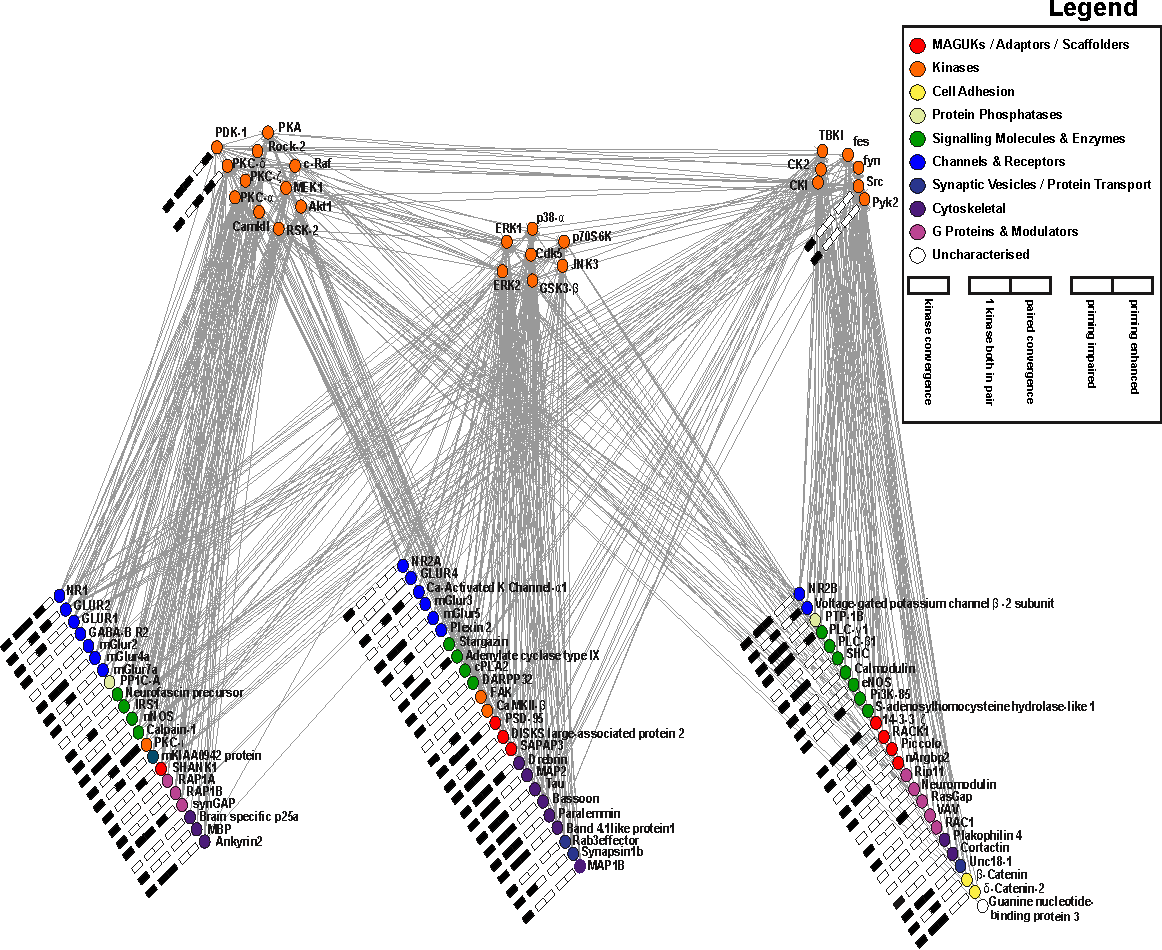
\includegraphics[height=6cm]{2000102CobaFig4.pdf}\citerrr{Coba2009phosphorylation}
 \end{center}
 %
 \note[item]{Molecular network, post-synaptic density, from Seth Grant}
 %
 \hyperlink{fr_questions}{There} is a complex, dynamical molecular network underlying synaptic plasticity.
 %
 \note[item]{Does this matter?}
 \note[item]{Could just be the machinery for changing synaptic weight}
 \note[item]{link back to questions on ``There''}
%
\end{frame}

%-------------Slide--------------------------------------------------------

\begin{frame}{Storage capacity of synaptic memory}
%
  A classical perceptron (used as a recognition memory device) has a capacity $\propto N$, the number of synapses.

 \vp Requires synapses' dynamic range also $\propto N$.

 \vp If we restrict synaptic weight to a fixed, finite set of values,\\
 \hp $\implies$ \parbox[t]{8cm}{tradeoff between learning and forgetting:\\
 new memories overwriting old.}
 %
 \note[item]{very plastic: learn easy, forget easy}
 \note[item]{little plasticity, remember better, learn harder}

 \vp If we wish to store new memories rapidly, memory capacity  $\sim\CO(\log N)$.
 \\ \citerr{amit1992constraints,amit1994learning}
 %
 \note[item]{or sparse $\sim \log N / N$}

 \vp To circumvent this tradeoff, need to go beyond model of a synapse as a single number.
 \note[item]{one way around limit: complexity}
%
\end{frame}

%-------------Section--------------------------------------------------------

\section{Modelling synaptic complexity}

%-------------Slide--------------------------------------------------------

\begin{frame}{Complex synapses}
%
  \aligntop{\includegraphics[width=5cm]{synapse.svg}}\hp
  %
  \note[item]{functional states, not molecules}
  \note[item]{synaptic weight depends on state}
  \note[item]{many states can have same weight}
  %
  \hp\aligntop{\includegraphics[width=2cm]{pot.svg}}
  \hp\aligntop{\includegraphics[width=2cm]{dep.svg}}
  %
  \note[item]{stochastic transitions}
%
\end{frame}

%-------------Slide--------------------------------------------------------

\begin{frame}{Simplifying assumptions}
%
\begin{itemize}
  \item There are $N$ identical synapses with $M$ internal functional states.
  \item States of different synapses are independent of each other.
      %
      \note[item]{allows us to concentrate on synapse, not neuron/network}
      %
  \item Which synapses eligible for plasticity chosen randomly.
      %
      \note[item]{don't care if STDP...}
      %
  \item Potentiating/depressing plasticity events $\sim$ Poisson processes with rates $rf\potdep$, where $f\pot+f\dep=1$.
      %
      \note[item]{$r=$ total rate of plasticity events per synapse, $f\potdep=$ fraction of events that are potentiating/depressing.}
      %
  \item Potentiation and depression are described by Markov processes with transition probabilities $\M\potdep$.
      %
      \note[item]{matrix elements: transition prob from $i\to j$, given pot/dep}
      %
  \item Synaptic weights of the internal states are given by vector $\w$.\\ Can only take values $\pm1$.
      %
      \note[item]{looks like binary synapse from outside. Inside...}
      \note[item]{ideal observer reads weights, not electrical activity: don't model neurons/network}
      \note[item]{upper bound on electrical activity readout}
\end{itemize}
%
\end{frame}

%-------------Slide--------------------------------------------------------

\begin{frame}{Dynamics}
%
 At $t=0$, the memory is created by $\M\potdep$ with probability $f\potdep$.
 \note[item]{for this one, we keep track of pot/dep, look for inc/dec of $\w$}

 \vp Forgetting caused by subsequent memories, evolving as
 %
 \begin{equation*}
   \diff{\pr(t)}{t} = r\pr(t)\frg,
   \qquad
   \frg = f\pot\M\pot+f\dep\M\dep-\I,
 \end{equation*}
 %
 \note[item]{$\frg$ is forgetting matrix, $\I=$identity, don't keep track of pot/dep}
 Eventually, this will settle into the equilibrium distribution:
 %
 \begin{equation*}
   \eq\frg=0.
 \end{equation*}
 %
 \note[item]{In equilibrium prior to memory creation}
%
\end{frame}

%-------------Slide--------------------------------------------------------

\begin{frame}{Memory curve}
%
 $\wv$ is the $N$-element vector of synaptic weights.
 %
 \note[item]{of different synapses}
 \note[item]{ideal observer reads weights, not states}
 \note[item]{upper bound on electrical activity readout}
 %
 \begin{equation*}
   \begin{aligned}
     \text{Signal} &= \av{\wv_\text{ideal} \cdot \wv(t) -  \wv_\text{ideal} \cdot \wv(\infty)}\\
     \text{Noise} &= \var\prn{\wv_\text{ideal} \cdot \wv(\infty)}
   \end{aligned}
 \end{equation*}
 %
 \note[item]{ideal: pot$\to$strong...}
 \note[item]{subtract baseline, some overlap even w/o encoding}
 \note[item]{if we ignore correlations...}
 %
 Related to reconstruction probability of single synapses.
 %
 \begin{equation*}
   \SNR(t) \sim \sqrt{N}\,P(\text{strong/weak},t|\text{pot/dep},t=0)-\ldots(t=\infty).
 \end{equation*}
 %

%
\end{frame}

%-------------Slide--------------------------------------------------------

\begin{frame}{Example models}
%
 Two example models of complex synapses.
 %
 \begin{center}
% \parbox[t]{30cm}{
  \aligntop{\includegraphics[width=4cm]{multistate.svg}}
  \hspace{2cm}
  \aligntop{\includegraphics[width=4cm]{cascade.svg}}
% }
 \end{center}
 \citerr{amit1994learning,Fusi2007multistate,Fusi2005cascade}
 %
 \note[item]{previous work, also: Benna-Fusi}

 These have different memory storage properties
 %
 \begin{center}
 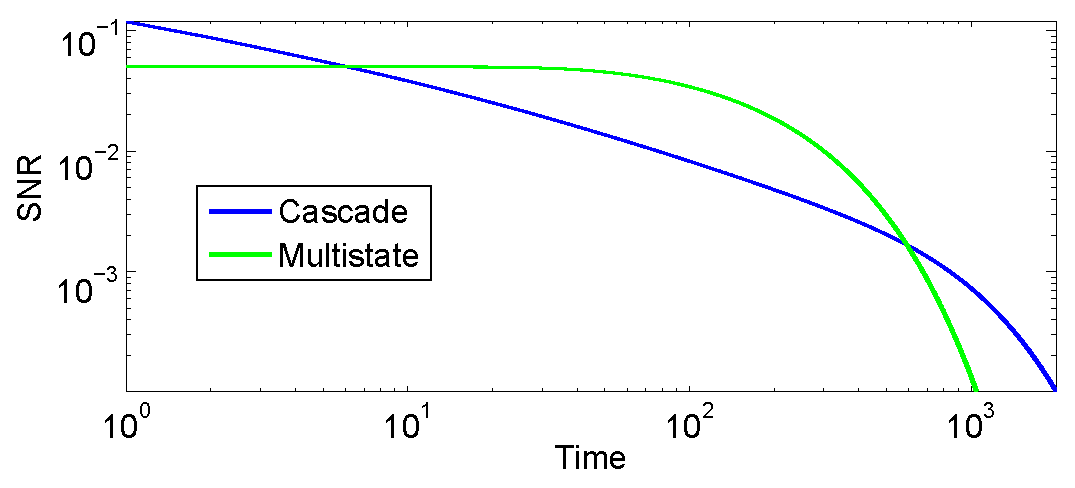
\includegraphics[width=8cm]{cascms.eps}
 \end{center}
 %
 \note[item]{Multistate good at one time, bad at others,}
 \note[item]{Cascade, less well at that time, better over range of times.}
%
\end{frame}

%-------------Slide--------------------------------------------------------

\begin{frame}[label=fr_questions]{Questions}
%
 \begin{itemize}
   \item Can we understand the space of \emph{all possible} synaptic models?
   \note[item]{not just individual models}
   \item How does structure \hyperlink{fr_net<1>}{(topology)} of model $\to$ function (memory curve)?
   \note[item]{understand net (link on topology)}
   \item What are the limits on what can be achieved?
   \note[item]{avoid using word ``optimal''. depends on what want to do.}
   \item Which transition topologies saturate these limits?
 \end{itemize}
%
\end{frame}

%-------------Slide--------------------------------------------------------

\begin{frame}{Memory curve 2}
%
 Memory curve given by
 %
 \begin{equation*}
   \snr(t) = \frac{\sqrt{N}(2f\pot f\dep)}{\sqrt{4\eq_+\eq_-}}\, \eq \prn{\M\pot-\M\dep}
      \exp\prn{rt\frg}\w.
 \end{equation*}
 %
 \note[item]{prefactors don't do anything, ignore}
 \note[item]{prior state, encoding, forgetting, readout}
 %
 Constraints: \qquad $\M\potdep_{ij}\in[0,1]$, \qquad $\sum_j\M\potdep_{ij}=1$.
 %
 \note[item]{difficult to to apply}

 \vp Eigenmode decomposition:
 %
 \begin{equation*}
   \snr(t) = \sqrt{N}\sum_a \initial_a \,\e^{-rt/\tau_a}.
 \end{equation*}
 %
 \note[item]{what are constraints on these?}
%
\end{frame}


%-------------Section--------------------------------------------------------

\section{Upper bounds}

%-------------Section--------------------------------------------------------

\subsection{Initial SNR}

%-------------Slide--------------------------------------------------------

\begin{frame}{Initial SNR as flux}
%
 Initial SNR is closely related to flux between strong \& weak states
 %
 \note[item]{flux = eq prob $\times$ trans prob}
 %
 \begin{equation*}
   \SNR(0) \leq \frac{4\sqrt{N}}{r}\,\F_{-+}.
 \end{equation*}
 %
 \note[item]{usually saturated: pot never dec, dep never inc}
 Max when {\parbox[t]{8cm}{potentiation guarantees $\w\to+1$,\\
 depression guarantees $\w\to-1$.}}
 %
 \begin{center}
   \includegraphics[height=3cm]{max_init_pot.svg}
   \hp \hp
   \includegraphics[height=3cm]{max_init_dep.svg}
 \end{center}
 %
 \note[item]{transitions out of one node sum to 1}
 \note[item]{equivalent to two-state model: doesn't matter which strong/weak state, same prob of going to other set.}
%
\end{frame}

%-------------Slide--------------------------------------------------------

\begin{frame}{Two-state model}
%
 Two-state model equivalent to previous slide:
  \begin{center}
  Transitions:
   \parbox{2cm}{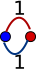
\includegraphics[height=2cm]{binary_det.svg}}
   $\implies\snr(t)=\sqrt{N}\,(4 f\pot f\dep)\,\e^{-rt}.$
  \end{center}
  \note[item]{decays very quickly}

 \vp Maximal initial SNR:\note[item]{$f\pot=\half$}
 %
 \begin{equation*}
   \snr(0) \leq \sqrt{N}.
 \end{equation*}
 %
 \note[item]{Initial SNR not a good thing to optimise.}
%
\end{frame}

%-------------Section--------------------------------------------------------

\subsection{Area under memory curve}

%-------------Slide--------------------------------------------------------

\begin{frame}{Area under memory curve}
%
  Memory lifetime bounded by area under SNR curve:\\
  \vp\parbox{5cm}{
  %
  \begin{equation*}
  \begin{aligned}
    \SNR(\text{lifetime})&=1
    \\
    \implies
    \quad
    \text{lifetime} &< \area.
  \end{aligned}
  \end{equation*}
  %
  }
  \parbox{6.5cm}{
    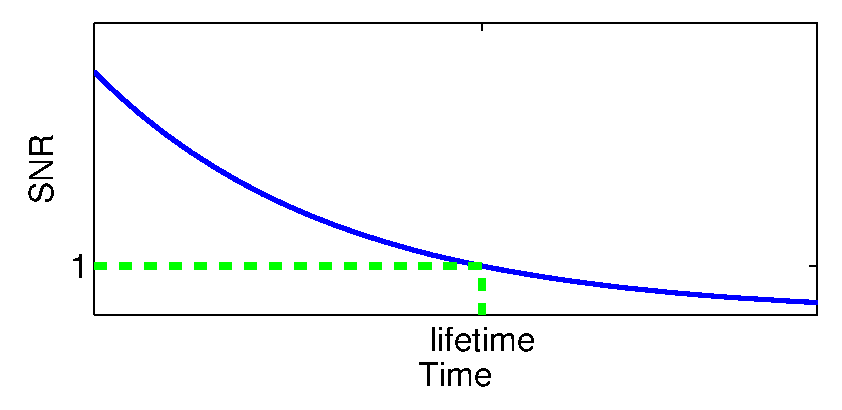
\includegraphics[width=6cm]{lifetime.eps}
  }
  %
  \note[item]{lifetime = area under green < area under blue}
  \note[item]{capacity $\sim r$ lifetime, \#new memories before we forget original.}

  %
  \vp This area has an upper bound:
  %
  \begin{equation*}
    \area \leq \sqrt{N}(M-1)/r.
  \end{equation*}
  %
  \note[item]{reminder: $N=$\#synapses, $M=$\#states}
  Saturated by a model with linear chain topology.
  \note[item]{proof next slide}
%
\end{frame}

%-------------Slide--------------------------------------------------------

\begin{frame}[label=fr_areaproof]{Proof of area bound}
%
 For any model, we can construct perturbations that
 \parbox[c]{5cm}{
  \begin{itemize}
    \item preserve equilibrium distribution,
    \item increase area.
  \end{itemize}
  \hyperlink{fr_tech}{\beamerbutton{details}}
  %
  \note[item]{relies on order \& technical condition}
 }
 \parbox[c]{5cm}{
  %
  \begin{center}
    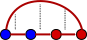
\includegraphics[width=4cm]{shortcut.svg}
  \end{center}
  %
 }\\
 \eg decrease``shortcut'' transitions, increase bypassed ``direct'' ones.\\
 Endpoint: linear chain

 \vp The area of this model is
 %
 \begin{equation*}
   A = \frac{2\sqrt{N}}{r}\sum_k \eq_k \abs{k-\av{k}}.
 \end{equation*}
 %
 \note[item]{max given $\eq$}
 \note[item]{now max \wrt $\eq$}
 Max: equilibrium probability distribution concentrated at both ends.
 \note[item]{keep c.o.m.\ in middle}
 \\
 \citerr{Barrett2008discrete}
 \note[item]{similar result, slightly different conditions: linear weights, mutual info}
%
\end{frame}

%-------------Slide--------------------------------------------------------

\begin{frame}{Saturating model}
%
 Make end states ``sticky''
 %
 \begin{center}
   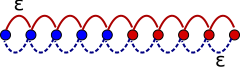
\includegraphics[width=8cm]{multistate_sticky.svg}
 \end{center}
 %
 Has long decay time, but terrible initial SNR.
 %
 \note[item]{Difficult to get out of end state.}
 \note[item]{Area not a good thing to optimise}
%
\end{frame}


%-------------Section--------------------------------------------------------

\section{Envelope memory curve}

%-------------Slide--------------------------------------------------------

\begin{frame}{Bounding finite time SNR}
%
 SNR curve:
 %
 \begin{equation*}
   \snr(t) = \sqrt{N}\sum_a \initial_a \,\e^{-rt/\tau_a}.
 \end{equation*}
 %
 \note[item]{from eigenmode decomposition}
 subject to constraints:
 %
 \begin{equation*}
   \sum_a \initial_a \leq 1,
   \qquad
   \sum_a \initial_a\, \tau_a \leq M-1.
 \end{equation*}
 %
 \note[item]{from initial, area bounds}
 We can maximise \wrt $\initial_a,\tau_a$.
%
\end{frame}


%-------------Slide--------------------------------------------------------

\begin{frame}{Constructing the envelope}
%
 %
 \begin{center}
 \begin{overlayarea}{10cm}{4.5cm}
   \only<1>{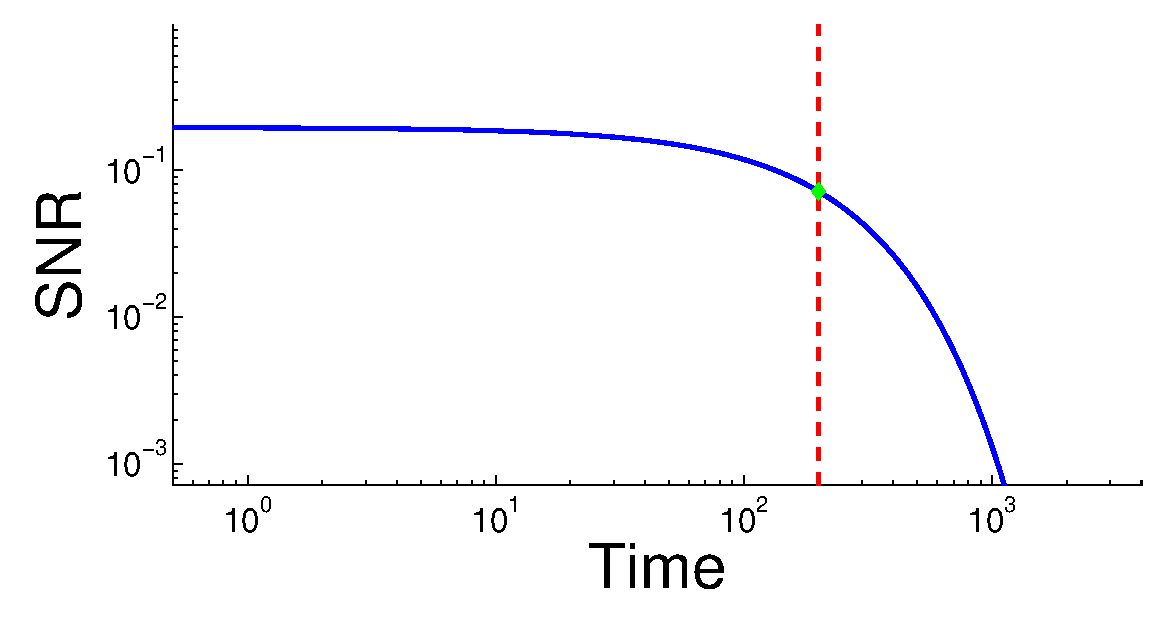
\includegraphics[width=8cm]{env2_t1.eps}}
   \only<2>{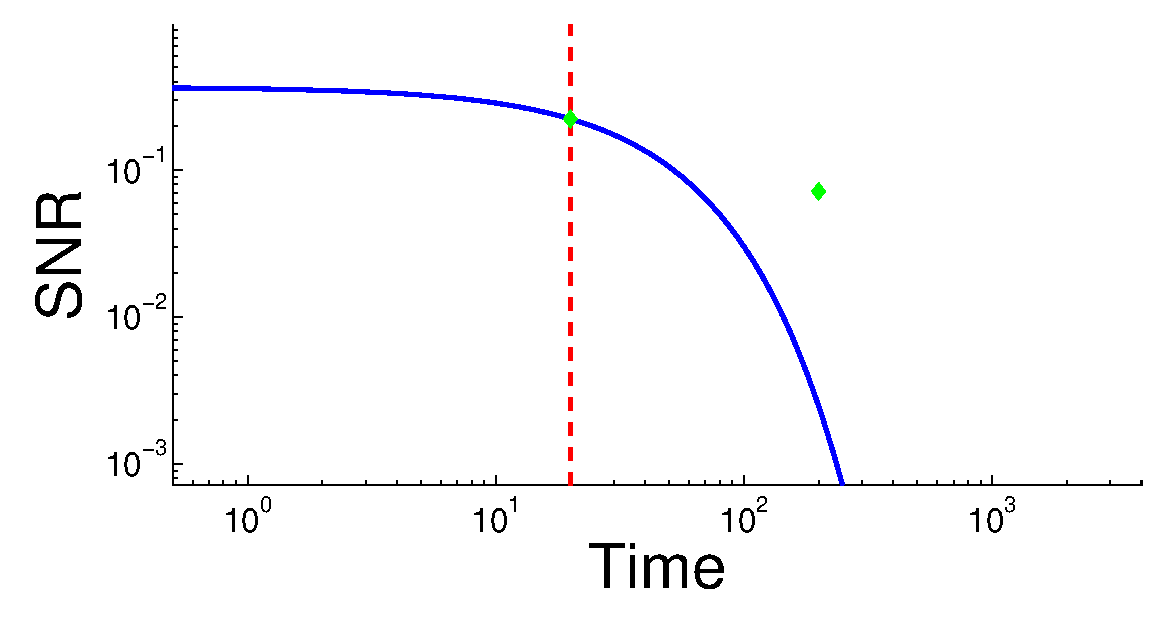
\includegraphics[width=8cm]{env2_t2.eps}}
   \only<3>{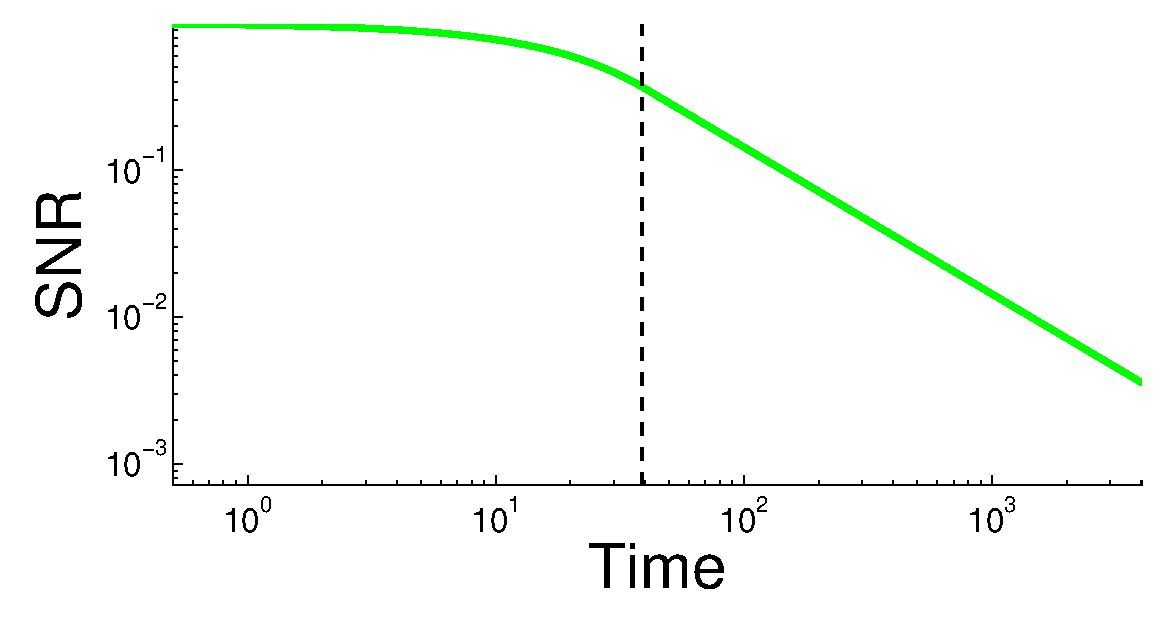
\includegraphics[width=8cm]{env2_all.eps}}
   \only<4>{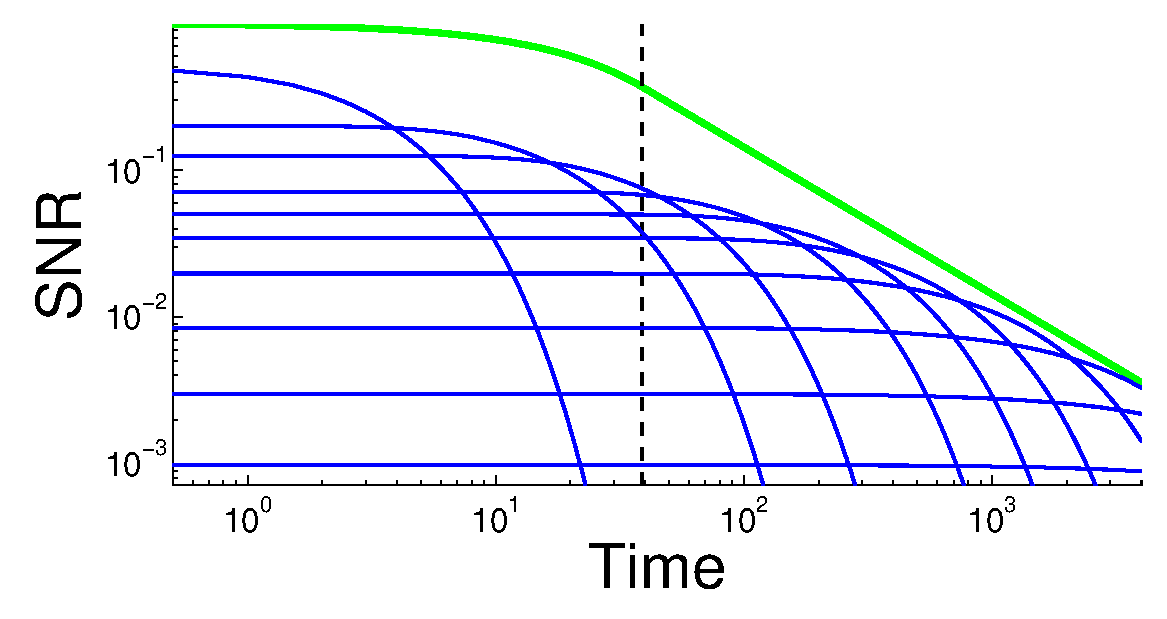
\includegraphics[width=8cm]{env2_ex.eps}}
 \end{overlayarea}
 \end{center}
 %
 \begin{overlayarea}{10cm}{2cm}
  \only<1>{Maximise SNR at one time}
  %
  \note<1->[item]{One exp. only constrains SNR at that time, not others}
  %
  \only<2>{Another time}
  %
  \note<2->[item]{get another bound}
  %
  \only<3>{All times $\to$ envelope}
  %
  \note<3->[item]{vary time of max. no curve can cross this.}
  \note<3->[item]{Regions: init(1); area(1,2)}
  \note<3->[item]{is it tight? can any constrained set of exps be acheived?}
  %
  \only<4>{Memory curves of example models.}
  %
  \note<4->[item]{no}
  \note<4->[item]{One exp. discuss models next slide}
 \end{overlayarea}
%
\end{frame}

%-------------Slide--------------------------------------------------------

\begin{frame}{Best models at single times}
%
 Early times:
 %
 \begin{center}
   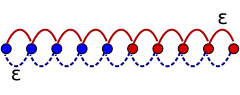
\includegraphics[width=6cm]{multistate_shorten.svg}
 \end{center}
 %
 \note[item]{shorten length of chain, keeping deterministic}
 %
 Late times:
 %
 \begin{center}
   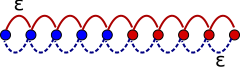
\includegraphics[width=6cm]{multistate_sticky.svg}
 \end{center}
 %
 \note[item]{Area maximising.}
 \note[item]{two mechs for slowing forgetting: time (lower trans prob) and space (diffusion length)}
 %
%
\end{frame}

%-------------Slide--------------------------------------------------------

\begin{frame}{Additional constraint}
%
 Conjecture: additional constraint
 %
 \begin{equation*}
   \initial_a\sqrt{\tau_a} \leq \CO(1).
 \end{equation*}
 %
 \note[item]{Tested experimentally. Discuss later}
 %
 Saturated by a diffusive chain:
 %
 \begin{equation*}
   \SNR(0) \sim \frac{1}{M},
   \qquad
   \text{time-scale} \sim M^2.
 \end{equation*}
 %
%
\end{frame}

%-------------Slide--------------------------------------------------------

\begin{frame}{Envelope 2}
%
 %
 \begin{center}
   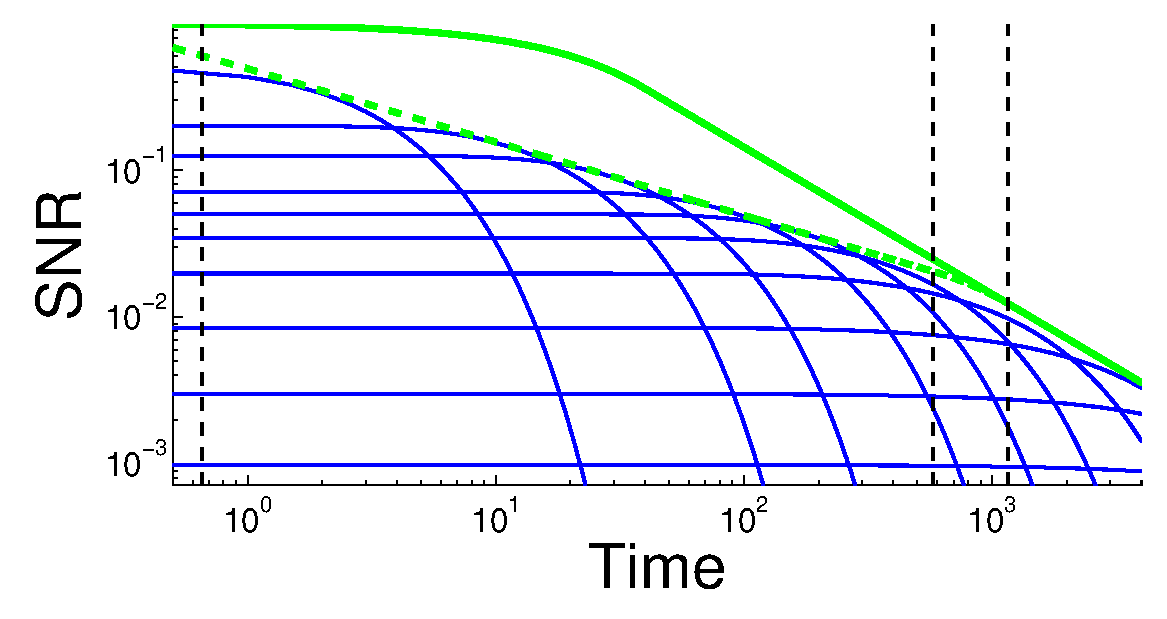
\includegraphics[width=8cm]{env23.eps}
 \end{center}
 %
 \note[item]{dashed: conjecture. tight.}

 %
 \begin{equation*}
 \begin{aligned}
   rt &< \CO(M^2), &\quad
   \text{envelope} &\sim (rt)^{-1/2}, \\
   rt &> \CO(M^2), &
   \text{envelope} &\sim (rt)^{-1} .
 \end{aligned}
 \end{equation*}
 %
 \note[item]{earlier: diffusion limited. later: stochastic limited.}
 \note[item]{regions: init(1); sqrt(2,3); area(3,4)}
 \note[item]{Benna-Fusi hugs envelope? cascade $\sim t^{-3/4}$}
%
\end{frame}

%-------------Slide--------------------------------------------------------

\begin{frame}{Lifetime bound}
%
 Lifetime of a memory bounded by where envelope crosses 1
 %
 \begin{equation*}
 \begin{aligned}
   N &> \CO(M^2) &\implies
   \text{lifetime} &\leq \frac{\sqrt{N}(M-1)}{\e r}, \\
   N &< \CO(M^2) &\implies
   \text{lifetime} &\leq \frac{\gamma^2{N}}{2\e r}.
 \end{aligned}
 \end{equation*}
 %
 \note[item]{$\gamma\sim\CO(1)$ constant in additional constaint}
 \note[item]{First $t^{-1}$ assumes M low. Second $t^{-1/2}$ applies to Benna-Fusi.}
 \note[item]{Independent synapses?}
%
\end{frame}

%-------------Slide--------------------------------------------------------

\begin{frame}{Additional constraint: other forms?}
%
 Involving eigenmodes:
 %
 \begin{equation*}
   \initial_a \sqrt{\tau_a},
   \qquad
   \sum_a \initial_a \sqrt{\tau_a},
   \qquad
   \sum_a \initial_a^2 {\tau_a}.
 \end{equation*}
 %
 \note[item]{as one-time max only involved one exp, would also work}
 \note[item]{right units}
 %
 Not involving eigenmodes
 %
 \begin{equation*}
   \area \times \snr(0),
   \qquad
   \intd{t} \snr(t)^2.
 \end{equation*}
 %
 \note[item]{easier to work with?}
 \note[item]{L2 doesn't have nice expression in terms of matrices}
%
\end{frame}

%-------------Slide--------------------------------------------------------

\begin{frame}{Cheeger inequality}
%
 \parbox{5cm}{
 Cheeger constant:
 %
 \begin{equation*}
   \phi \equiv \min_\CS \brc{\frac{\operatorname{Perimeter}(\p\CS)}{\operatorname{Area}(\CS)}}.
 \end{equation*}
 %
 \note[item]{split into two pieces. pick smaller. higher dim.}
 \note[item]{bottleneck}
 }
 \parbox{6cm}{
   \includegraphics[width=5cm]{dumbbell.svg}
 }
 Timescale for diffusion to equilibriate
 %
 \begin{equation*}
   \frac{1}{D \tau_{\text{diffusion}}} > \CO(1)\, \phi^2.
 \end{equation*}
 %
 \note[item]{if we want slow diffusion, need lhs small $\to$ need bottleneck.}
 \note[item]{purely geometric}
 \note[item]{also inequality in other direction: want slow diffusion $\to$ need bottleneck. Not useful for us}
%
\end{frame}

%-------------Slide--------------------------------------------------------

\begin{frame}{Cheeger inequality: Markov chains}
%
 Cheeger constant:
 %
 \begin{equation*}
   \phi \equiv \min_\CS \brc{\frac{\F_{\CS\CS\comp}}{\eq(\CS)}}.
 \end{equation*}
 %
 \note[item]{split states into two subsets. pick smaller.}
 \note[item]{again bottleneck}
 \note[item]{denominator varies}
 %
 Timescale to equilibriate:
 %
 \begin{equation*}
   \frac{1}{\max_a\tau_a} > \CO(1)\, \phi^2.
 \end{equation*}
 %
 Simple proof assuming detailed balance. \citerr{Sinclair1989cheeger}\\
 More complicated proof for general case. \citerr{Lawler1988cheeger}
 %
 \note[item]{$\CO(1)$ bit differs}
 \note[item]{bottleneck need not be between strong \& weak.}
%
\end{frame}

%-------------Slide--------------------------------------------------------

\begin{frame}{Counter examples?}
%
 Put bottleneck somewhere else:
 %
 \begin{center}
   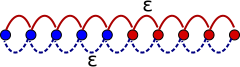
\includegraphics[width=6cm]{multistate_counter.svg}
 \end{center}
 %
 \note[item]{eq prob concentrated near middle. bottleneck at $\epsilon$.}
 %
 Set $\epsilon = 1/M$, see how putative constraints vary:
 %
 \begin{center}
   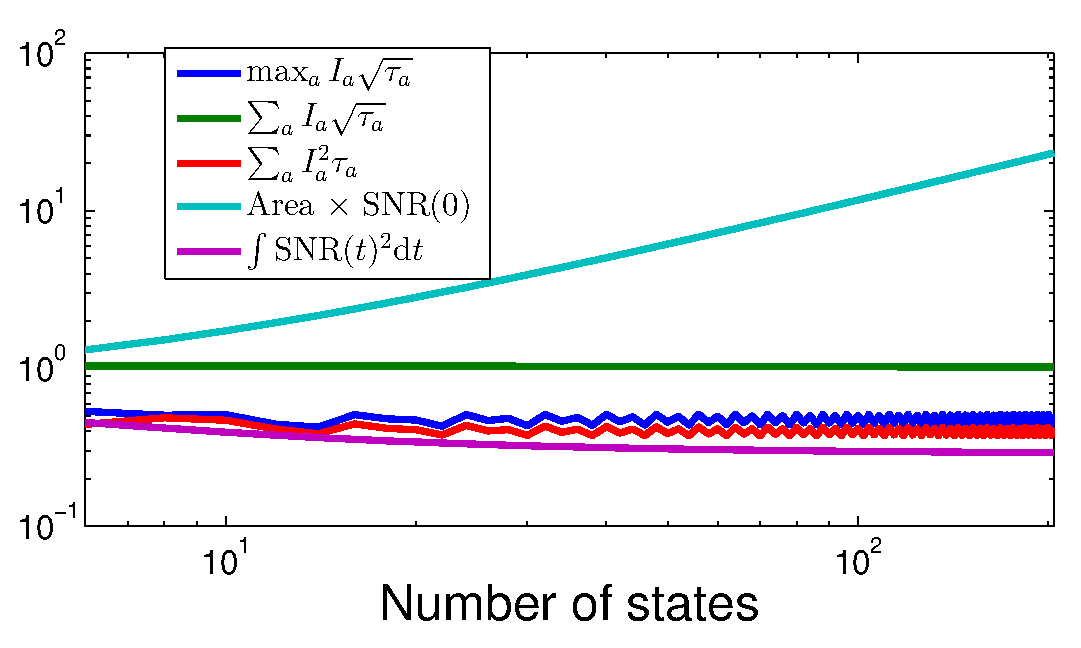
\includegraphics[width=6cm]{counter_graph.eps}
 \end{center}
 %
 \note[item]{high inital snr and long timescale in different modes.}
 \note[item]{only eigenmode dependent constraints survive (and L2 - but difficult to work with).}

 Also tried: random Markov chains.
%
\end{frame}

%-------------Slide--------------------------------------------------------

\begin{frame}{Two-time envelope}
%
 Maximise $\snr(t_1)$ subject to constraint $\snr(t_2)=S_2$.
 %

 \vp For $t_1$ close to $t_2$, get single exponential. Far away, get two exponentials.
 %
 \note[item]{Max at multiple times, $\to$ multiple timescales? cascade? Benna-Fusi?}

 \vp See tradeoff between $\snr(t_1)$ and $\snr(t_2)$.
 %

 %
 \begin{center}
   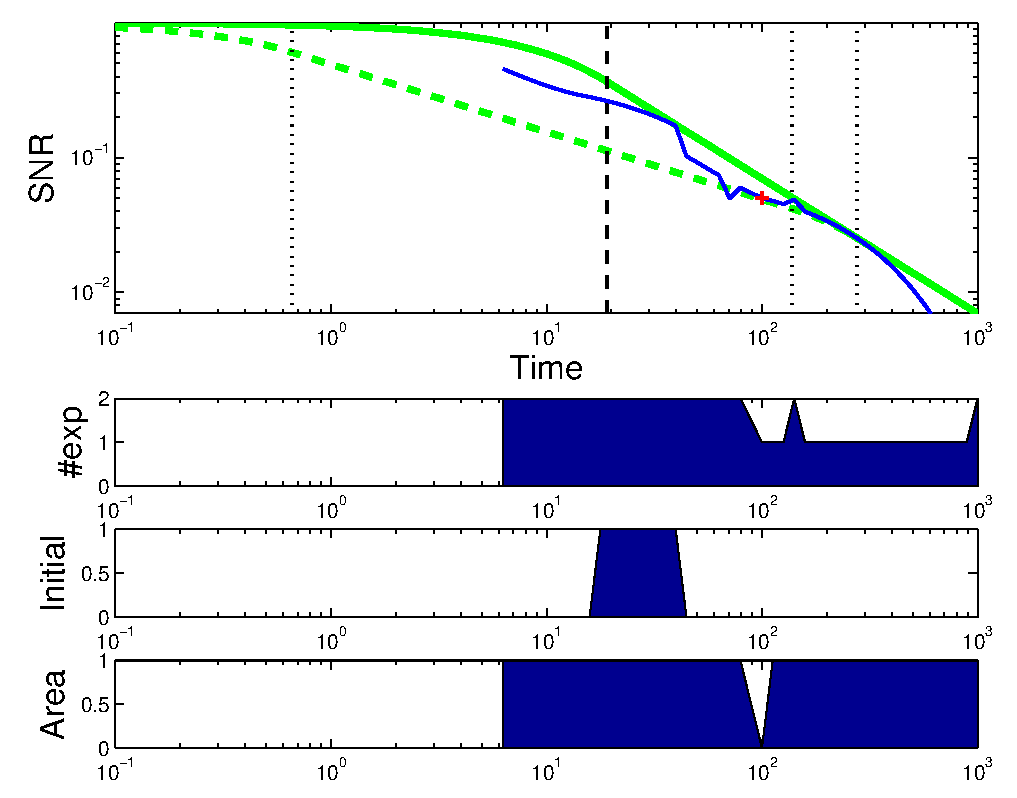
\includegraphics[width=5cm]{two_time_env.eps}
 \end{center}
 %
\note[item]{only implemented first 2 constraints}
  \note[item]{numerics not working. 2 exp solution need to solve 2 transcendental equations.}
%
\end{frame}

%-------------Slide--------------------------------------------------------

\begin{frame}{Summary}
%
  \begin{itemize}
    \item We have formulated a general theory of learning and memory with complex synapses.
%    \item We can impose an order on the internal states of a synapse through the theory of first passage times.
    \item The area under the memory curve of any model $<$ linear chain with same equilibrium distribution.
    \item We find a memory envelope: a single curve that cannot be exceeded by the memory curve of \emph{any} synaptic model.
    \item Synaptic complexity ($M$ internal states) raises the memory envelope linearly in $M$ for times $> \CO(M^2)$.
    \item For times $< \CO(M^2)$: conjecture that the model that reaches the envelope uses deterministic transitions $\to$ diffusive forgetting.
  \end{itemize}

%
\end{frame}





%-------------Slide--------------------------------------------------------
%
%% Press Ctrl-D to insert a new slide
%
%
%-------------Slide--------------------------------------------------------

\begin{frame}{Acknowledgements}
%
 Thanks to:
 \begin{itemize}
   \item Surya Ganguli
   \item Stefano Fusi
   \item Marcus Benna
 \end{itemize}
 \note[item]{Last slide!}
%
\end{frame}

%-------------Slide--------------------------------------------------------

\begin{frame}[allowframebreaks]{References}
%

 {\small
 \bibliographystyle{unsrt_slides}
 \bibliography{maths,neuro}
 }
%
\end{frame}

%-------------Slide--------------------------------------------------------

\begin{frame}[label=fr_tech]{Techinical detail: ordering states}
%
 Let $\fpt_{ij}=$ mean first passage time from state $i$ to state $j$.
 Then:
 %
 \begin{equation*}
   \eta = \sum_j \fpt_{ij} \eq_j,
 \end{equation*}
 %
 is independent of the initial state $i$
 (Kemeney's constant).\\ \citerr{kemeny1960finite}

 \vp We define:
 %
 \begin{equation*}
   \eta^+_i = \sum_{j\in\text{strong}} \fpt_{ij} \eq_j,
   \qquad
   \eta^-_i = \sum_{j\in\text{weak}} \fpt_{ij} \eq_j.
 \end{equation*}
 %
 \note[item]{Measure ``distance'' to the strong/weak states.}
 They can be used to arrange the states in an order (increasing $\eta^-$ or decreasing $\eta^+$).
 \hyperlink{fr_areaproof}{\beamerbutton{back}}
 \note[item]{sum to constant, $\implies$ two orders same}
%
\end{frame}

%-------------Slide--------------------------------------------------------

\begin{frame}{Technical detail: upper/lower triangular}
%
 With states in order:
 %
 \begin{center}
   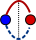
\includegraphics[width=2cm]{triangular_right.svg}
   \hp \hp \hp
   \includegraphics[width=2cm]{triangular_left.svg}
 \end{center}
 %
 \note[item]{pot \& dep with same initial \& final state}
 Endpoint: potentiation goes right, depression goes left.
 \note[item]{pot/dep matrices are upper/lower triangular.}
 \note[item]{one other pert. too technical, even for bonus slide!}

 \hyperlink{fr_areaproof}{\beamerbutton{back}}
%
\end{frame}


%-----End----------------------------------------------------------------

\end{document}
